%\documentclass[12pt, hyperref={pdfpagemode=FullScreen} ]{beamer}
\documentclass[12pt]{beamer}

\usepackage{lmodern}
\usepackage{array}
\usepackage{color}
\usepackage{listings}
\usepackage{minted}
\usemintedstyle{autumn}


\renewcommand{\theFancyVerbLine}{\sffamily
\textcolor[rgb]{0.5,0.5,1.0}{\scriptsize
\oldstylenums{\arabic{FancyVerbLine}}}}


\mode<presentation>
{
	%\usetheme{Warsaw}
	%\usetheme{Darmstadt}
	\usetheme{Boadilla}
	%\usetheme{CambridgeUS}
	%\usetheme{Madrid}
}

\makeatletter
\setbeamertemplate{footline}
{
  \leavevmode%
  \hbox{%
  \begin{beamercolorbox}[wd=.333333\paperwidth,ht=2.25ex,dp=1ex,center]{author in head/foot}%
    \usebeamerfont{author in head/foot}\insertshortauthor%~~\beamer@ifempty{\insertshortinstitute}{}{(\insertshortinstitute)}
  \end{beamercolorbox}%
  \begin{beamercolorbox}[wd=.333333\paperwidth,ht=2.25ex,dp=1ex,center]{title in head/foot}%
    \usebeamerfont{title in head/foot}\insertshorttitle
  \end{beamercolorbox}%
  \begin{beamercolorbox}[wd=.333333\paperwidth,ht=2.25ex,dp=1ex,right]{date in head/foot}%
    \usebeamerfont{date in head/foot}\insertshortdate{}\hspace*{2em}
    \insertframenumber{} / \inserttotalframenumber\hspace*{2ex} 
  \end{beamercolorbox}}%
  \vskip0pt%
}
\makeatother



\def\newblock{\hskip .11em plus.33em minus.07em} %to solve a beamer problem with bib files

\usepackage{times}
\usepackage{tikz}
\usepackage{verbatim}
\usetikzlibrary{arrows,shapes}
\usepackage{natbib} 


\setbeamertemplate{navigation symbols}{
   %\insertslidenavigationsymbol
   %\insertframenavigationsymbol
   %\insertsubsectionnavigationsymbol
   %\insertsectionnavigationsymbol
   %\insertdocnavigationsymbol
   %\insertbackfindforwardnavigationsymbol
}
\title[Ruby on Rails]{Subversion}
\date{}
\institute{}
\author{Pierre-Yves Dupont}
\begin{document}


\newcommand{\mynewsection}[1]{
\section{#1}
\subsection*{}
\begin{frame}
	\begin{block}{}
		\center{#1}
	\end{block}
\end{frame}
}

\begin{frame}
	\titlepage
\end{frame}

\mynewsection{Introduction}

\begin{frame}
	\begin{block}{What is subversion}
		\begin{itemize}[<+->]
		  \item SVN (2000). Last version 1.7.6 (August, 15 2012)
		  \item revision control system (version control)
		  \item CVS 1986, Hg (Mercurial) 2005, Git 2005
		\end{itemize}
	\end{block}
\end{frame}

\begin{frame}
	\begin{block}{SVN System}
		\centering{
			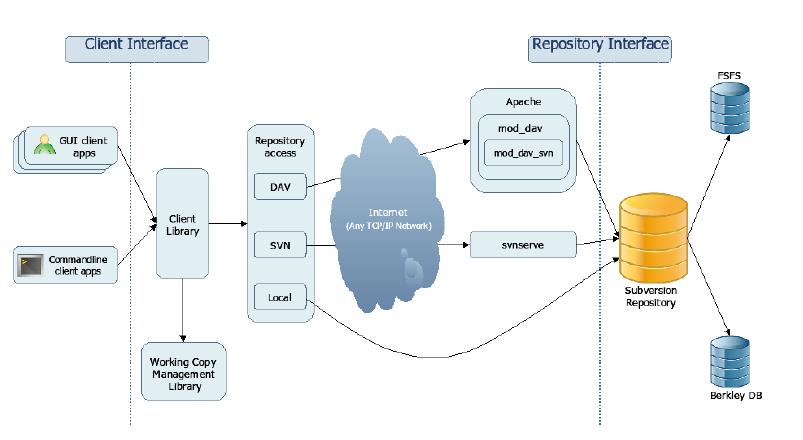
\includegraphics[scale=0.4]{img/architecture_svn.jpg}
		}
	\end{block}
\end{frame}

\begin{frame}
	\begin{block}{Problem}
		\centering{
				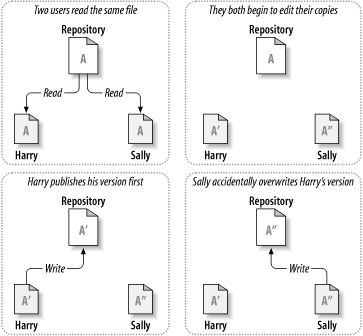
\includegraphics[scale=0.4]{img/overwriting.png}
			}
	\end{block}
\end{frame}

\begin{frame}
	\begin{block}{SVN solution}
		\only<1>{
			\centering{
					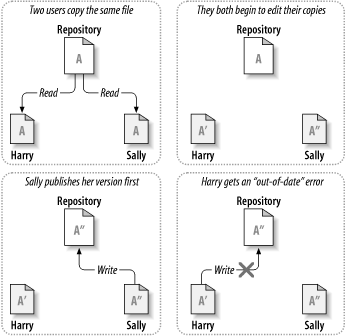
\includegraphics[scale=0.4]{img/merge1.png}
				}
		}
		\only<2>{
			\centering{
					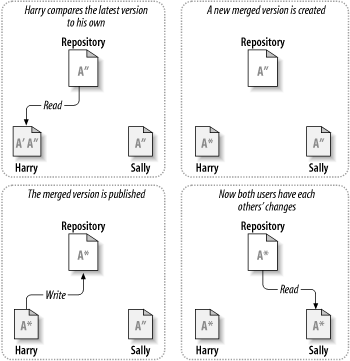
\includegraphics[scale=0.4]{img/merge2.png}
				}
		}
	\end{block}
\end{frame}

\mynewsection{SVN commands}

\begin{frame}
	\begin{block}{SVN workflow}
		\centering{
			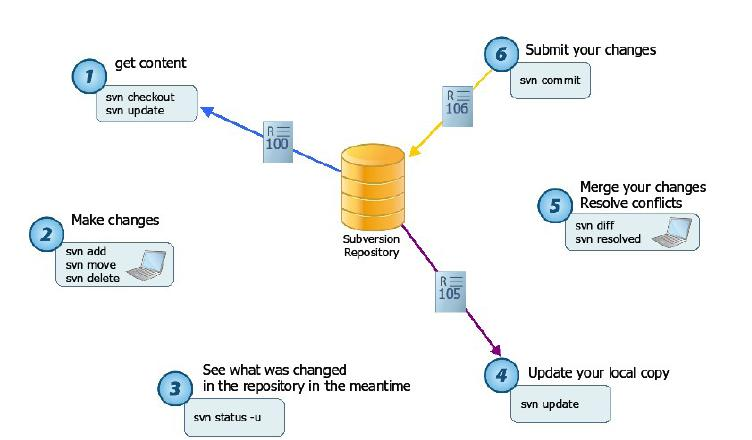
\includegraphics[scale=0.4]{img/svn_pipeline.jpg}
		}
	\end{block}
\end{frame}

\begin{frame}[fragile]
	\begin{block}{Proxy configuration}
		Edit the file:
		\begin{minted}[fontsize=\scriptsize]{bash}
~/.subversion/servers
		\end{minted}
		Find the ``[global]'' section and uncomment the following lines:
		\begin{minted}[fontsize=\scriptsize]{bash}
[global]
http-proxy-host = tur-cache1.massey.ac.nz
http-proxy-port = 8080
http-proxy-username = <user name>
http-proxy-password = <password>
		\end{minted}
Save the correct informations
	\end{block}
\end{frame}

\begin{frame}[fragile]
	\begin{block}{Getting the data: checkout}
		\begin{minted}[fontsize=\scriptsize]{bash}
%> svn checkout --username "username" \
	 --password "pwd" http://mysvn.com/repository
		\end{minted}
		No need to put the password in the command line\\
		Same as:
		\begin{minted}[fontsize=\scriptsize]{bash}
%> svn co --username "username" http://mysvn.com/repository
		\end{minted}
	\end{block}
	\begin{exampleblock}{checkout}
		 Pull an SVN tree from the server. Should be done only once.
	\end{exampleblock}
\end{frame}

\begin{frame}[fragile]
	\begin{block}{Updating the data: update}
		The command must be launched in the directory to update. Or give the path of the directory
		\begin{minted}[fontsize=\scriptsize]{bash}
%> svn update
		\end{minted}
		Same as:
		\begin{minted}[fontsize=\scriptsize]{bash}
%> svn up
		\end{minted}
		The informations about the repository, the user, etc\ldots are in the .svn directory.
	\end{block}
	\begin{exampleblock}{update}
		 Synchronize your local copy with the server: add the new files, delete the removed files, merge the modified files.
	\end{exampleblock}
\end{frame}

\begin{frame}[fragile]
	\begin{block}{Make changes on svn tree: add, move, \ldots}
		\begin{minted}[fontsize=\scriptsize]{bash}
%> svn add FILE_OR_DIR
%> svn move SRC DEST
%> svn mkdir DIR
		\end{minted}
	\end{block}
	\begin{block}{Delete files or directories}
		\begin{minted}[fontsize=\scriptsize]{bash}
%> svn delete FILE_OR_DIR
%> svn remove FILE_OR_DIR
%> svn del FILE_OR_DIR
%> svn rm FILE_OR_DIR
		\end{minted}
		Same command
	\end{block}
	\begin{exampleblock}{add move delete mkdir}
		 Use the svn commands to act on files and directories in your local copy
	\end{exampleblock}
\end{frame}

\begin{frame}[fragile]
	\begin{block}{Sending the changes to the repository: commit}
		\begin{minted}[fontsize=\scriptsize]{bash}
%> svn commit files_or_dirs_to_commit -m 'a comment please!'
		\end{minted}
		Same as:
		\begin{minted}[fontsize=\scriptsize]{bash}
%> svn ci files_or_dirs_to_commit -m 'a comment please!'
		\end{minted}
	\end{block}
	\begin{exampleblock}{commit}
		 Commit your local copy with all the changes you made on the repository. Don't forget to update first!
	\end{exampleblock}
\end{frame}

\begin{frame}[fragile]
	\begin{block}{get informations: status}
		\begin{minted}[fontsize=\scriptsize]{bash}
%> svn status -uv FILE_OR_DIR
		\end{minted}
		Same as:
		\begin{minted}[fontsize=\scriptsize]{bash}
%> svn st -uv FILE_OR_DIR
		\end{minted}
'u' option is used to compare the files with the repository, 'v' is used to display all files and directories even if they are up to date.
	\end{block}
	\begin{exampleblock}{status}
		 Obtaining informations about the status of files or directories. The status of each file is given by a letter: added (A), deleted (D), conflicted (C), Ignored (I), modified (M), unversioned (?), missing (!), up to date ( )
	\end{exampleblock}
\end{frame}

\mynewsection{Examples}

\begin{frame}[fragile]
	\begin{block}{svn co}
		\begin{minted}[fontsize=\scriptsize]{bash}
%>svn co file:///var/svn/projet1
A    projet1/foo
Checked out revision 11.
		\end{minted}
	\end{block}
	\begin{block}{svn status}
		\begin{minted}[fontsize=\scriptsize]{bash}
%>svn status -uv
M               11        8 pydupont     foo
                11       11 pydupont     .
Status against revision:     11
		\end{minted}
	\end{block}
\end{frame}

\begin{frame}[fragile]
	\begin{block}{svn log -v}
		\begin{minted}[fontsize=\scriptsize]{bash}
r7 | pydupont | 2012-09-13 15:02:05 +1200 (Thu, 13 Sep 2012) | 1 line
Changed paths:
   D /bar

delete one file
------------------------------------------------------------------------
r6 | pydupont | 2012-09-13 15:01:15 +1200 (Thu, 13 Sep 2012) | 1 line
Changed paths:
   A /baz

add one file
------------------------------------------------------------------------
r5 | pydupont | 2012-09-13 14:53:15 +1200 (Thu, 13 Sep 2012) | 1 line
Changed paths:
   M /foo

conflict resolved
------------------------------------------------------------------------
		\end{minted}
	\end{block}
\end{frame}

\begin{frame}[fragile]
	\begin{block}{svn add, svn up, svn commit}
		\begin{minted}[fontsize=\scriptsize]{bash}
%>touch bar
%> svn add bar
A         bar
%> svn up
At revision 11.
%> svn ci -m "add bar"
Adding         bar
Transmitting file data .
Committed revision 12.
		\end{minted}
	\end{block}
\end{frame}

\mynewsection{The conflicts}

\begin{frame}[fragile]
	\begin{block}{What is a conflict}
	A conflict occurs when there is two different modifications (by two users) on a same line in the same file
	\end{block}
	\begin{block}{}
	\begin{minted}[fontsize=\scriptsize]{bash}
%>svn update
Conflict discovered in 'foo'.
Select: (p) postpone, (df) diff-full, (e) edit,
        (mc) mine-conflict, (tc) theirs-conflict,
        (s) show all options: p 
C    foo
Updated to revision 4.
Summary of conflicts:
  Text conflicts: 1
		\end{minted}
	\end{block}
\end{frame}

\begin{frame}[fragile]
	\begin{block}{What is a conflict}
		\begin{minted}[fontsize=\scriptsize]{bash}
%>svn status -uv
C                4        4 pydupont     foo
?                                        foo.r3
?                                        foo.r4
?                                        foo.mine
                 4        4 pydupont     .
Status against revision:      4
		\end{minted}
	\end{block}
	\begin{block}{foo}
		\begin{minted}[fontsize=\scriptsize]{bash}
%>more foo
<<<<<<< .mine
First line - conflict
=======
Other line
>>>>>>> .r4
Second line
		\end{minted}
	\end{block}
	\begin{exampleblock}{Solution}
		Conpare the files
	\end{exampleblock}
\end{frame}

\begin{frame}[fragile]
	\begin{block}{foo}
		\begin{minted}[fontsize=\scriptsize]{bash}
%>more foo
<<<<<<< .mine
First line - conflict
=======
Other line
>>>>>>> .r4
Second line
		\end{minted}
	\end{block}
	\begin{block}{foo.r4}
		\begin{minted}[fontsize=\scriptsize]{bash}
%>more foo.r4
Other line
Second line
		\end{minted}
	\end{block}
	\begin{block}{foo.mine}
		\begin{minted}[fontsize=\scriptsize]{bash}
%>more foo.mine 
First line - conflict
Second line
		\end{minted}
	\end{block}
	\only<2>{
	\begin{exampleblock}{Solution}
		Conpare the files
	\end{exampleblock}
	}
\end{frame}

\mynewsection{Comparing files}

\begin{frame}[fragile]
	\begin{block}{Tools to compare the files}
		\begin{itemize}[<+->]
		  \item command lines: svn diff, diff \ldots
		  \item GUI: xxdiff, gvim -d, meld, \ldots
		  \item In Eclipse: Subclipse
		\end{itemize}
	\end{block}
\end{frame}

\begin{frame}[fragile]
	\begin{block}{Meld: display the conflicted files}
		\centering{
			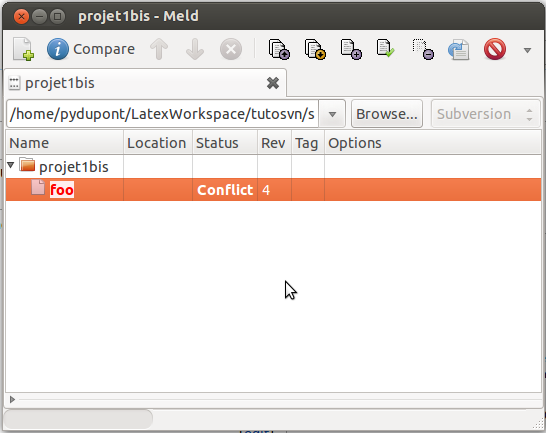
\includegraphics[scale=0.4]{img/meldconflict.png}
		}
	\end{block}
\end{frame}

\begin{frame}[fragile]
	\begin{block}{Meld: edit the conflited files}
		\centering{
			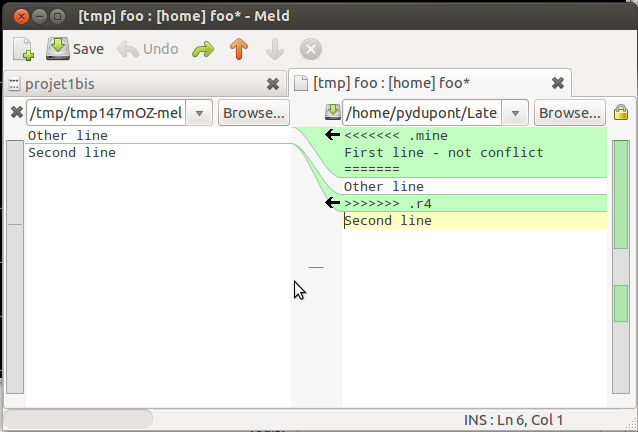
\includegraphics[scale=0.4]{img/meldeditconflict.png}
		}
	\end{block}
\end{frame}

\begin{frame}[fragile]
	\begin{block}{Meld: resolve the conflicts}
		\centering{
			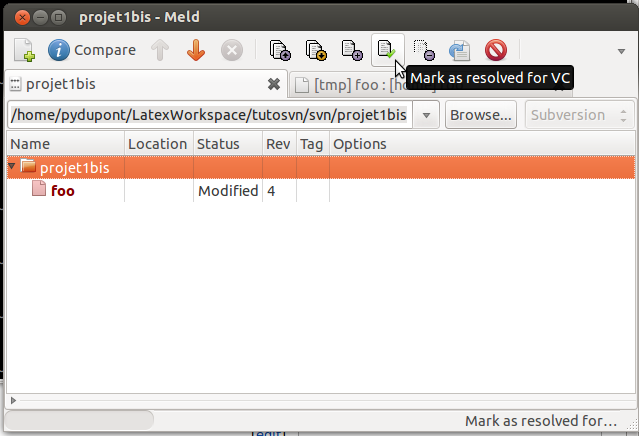
\includegraphics[scale=0.4]{img/meldconflictresolved.png}
		}
	\end{block}
\end{frame}


\begin{frame}[fragile]
	\begin{block}{Meld: commit}
		\centering{
			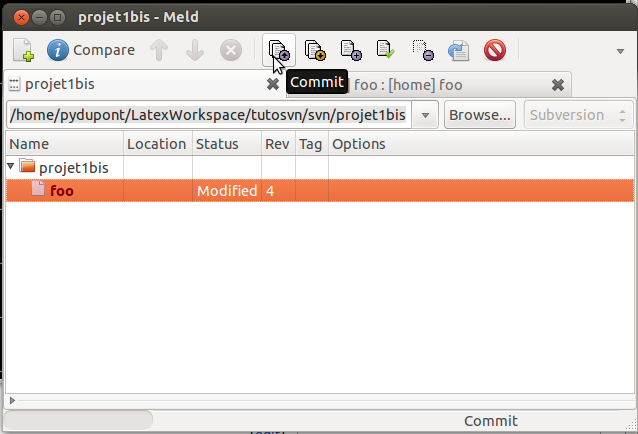
\includegraphics[scale=0.4]{img/meldcommit.png}
		}
	\end{block}
\end{frame}

\begin{frame}[fragile]
	\begin{block}{Meld: add a log message to the commit}
		\centering{
			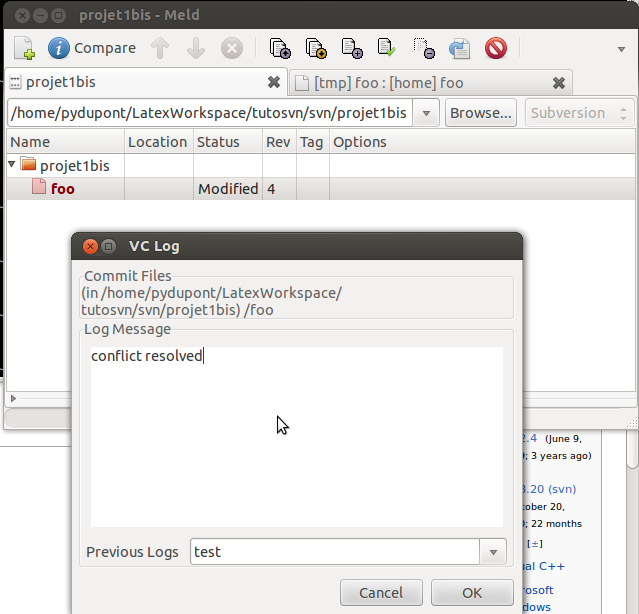
\includegraphics[scale=0.4]{img/meldlog.png}
		}
	\end{block}
\end{frame}

\begin{frame}[fragile]
	\begin{block}{Meld: update}
		\centering{
			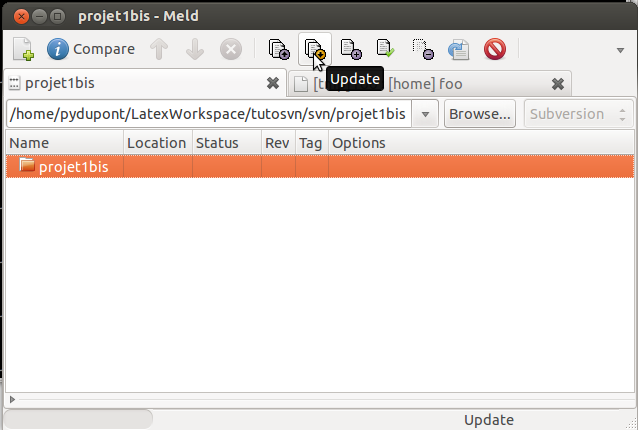
\includegraphics[scale=0.4]{img/meldupdate.png}
		}
	\end{block}
\end{frame}




\mynewsection{Setup your own svn repository}

\begin{frame}[fragile]
	\begin{block}{Make a folder for the new repository}
		\begin{minted}[fontsize=\scriptsize]{bash}
%>sudo mkdir /var/svn
		\end{minted}
	\end{block}
\end{frame}

\begin{frame}[fragile]
	\begin{block}{Start svn server with your system}
		\begin{minted}[fontsize=\scriptsize]{bash}
%>sudo gedit /etc/init.d/svnserve
		\end{minted}
		\end{block}
		\begin{block}{}
		\begin{minted}[fontsize=\tiny, linenos, numbersep=5pt]{bash}
#!/bin/sh
do_start () {svnserve -d -r /var/svn --pid-file /var/run/svnserve.pid}
do_stop () {start-stop-daemon --stop --quiet --pidfile /var/run/svnserve.pid}
case "$1" in
	start)
  		do_start
 		;;
 	stop)
 		do_stop
 		exit $?
 		;;
 	restart)
 		do_stop
		sleep 1s
 		do_start
 		;;
	reload|force-reload)
		echo "Error: argument '$1' not supported" >&2
		exit 3
		;;
	*)
		echo "Usage: $0 start|stop|restart" >&2
		exit 3
		;;
esac
		\end{minted}
		Change line 2 to setup the correct location
	\end{block}
\end{frame}

\begin{frame}[fragile]
	\begin{block}{Start svn server with your system}
		\begin{minted}[fontsize=\scriptsize]{bash}
%>sudo chmod +x /etc/init.d/svnserve
%>sudo update-rc.d svnserve defaults
%>sudo /etc/init.d/svnserve start
		\end{minted}
	\end{block}
\end{frame}

\begin{frame}[fragile]
	\begin{block}{Create a repository}
		\begin{minted}[fontsize=\scriptsize]{bash}
%>sudo svnadmin create /var/svn/my_repository_name
		\end{minted}
	\end{block}
	\begin{block}{Setup the repository}
		Uncomment the following lines in file 
		\begin{minted}[fontsize=\scriptsize]{bash}
		/repository/path/conf/svnserve.conf
		\end{minted}
		\hline
		\begin{minted}[fontsize=\scriptsize]{bash}
anon-access = none
auth-access = write
password-db = passwd
		\end{minted}
	\end{block}
	\begin{block}{Setup the access to repository}
		Edit the file 
		\begin{minted}[fontsize=\scriptsize]{bash}
		/repository/path/conf/passwd
		\end{minted}
		\hline
		\begin{minted}[fontsize=\scriptsize]{bash}
[users]
user1_login = user1_password
user2_login = user2_password
		\end{minted}
	\end{block}
\end{frame}

\mynewsection{Documentation}

\begin{frame}
	\begin{block}{web sites}
		\tiny{
		Ubuntu:
		\begin{enumerate}
		  \item RabbitVCS \url{http://wiki.rabbitvcs.org/wiki/install/ubuntu}
		  \item SVN book \url{http://svnbook.red-bean.com/en/1.7/svn-book.html}
		  \item Wikipedia \url{http://en.wikipedia.org/wiki/Apache_Subversion}
		  \item Ubuntu doc \url{https://help.ubuntu.com/community/Subversion}
		\end{enumerate}
		MAC OSX:
	  	\begin{itemize}
	  	  \item Installation \url{http://www.rubyrobot.org/tutorial/subversion-with-mac-os-x}
	  	  \item GUI \url{http://www.lachoseinteractive.net/en/community/subversion/svnx/features/}
	  	\end{itemize}
		}
	\end{block}
\end{frame}

\end{document}
